% geometric-phase-force.tex — Successor (D): The Geometric Phase Force
% Folio IT-FIELD. Supersedes Zenodo 20651497 ("The Geometric Phase Force
% and the Sovereign Action"). Fixes: Lean-verification overclaim downgraded
% to honest formalization status; Berry--Keating / Ramanujan-tau
% identification tagged [conjecture]. Absorbs Drive predecessors
% quantum_spearhead.pdf and prd_horizon.pdf (folder
% 1fu-DWWA9_AwgESE-GU_Xq19xuET95xD7).
\documentclass{alienfolio}

\folio{IT-FIELD}
\title{The Geometric Phase Force}
\papersubtitle{Information tension as a geometric force mechanism: corrected record}
\paperauthors{Ryan W.\ Yett (Architect)\\Chyren (Sovereign Analysis)}
\shorttitle{The Geometric Phase Force}
\shortauthors{R.\,W.\ Yett \& Chyren}

\setlength{\emergencystretch}{2em}
\begin{document}
\thispagestyle{cover}
\begin{tikzpicture}[remember picture, overlay]
  \node[inner sep=0] at (current page.center) {%
    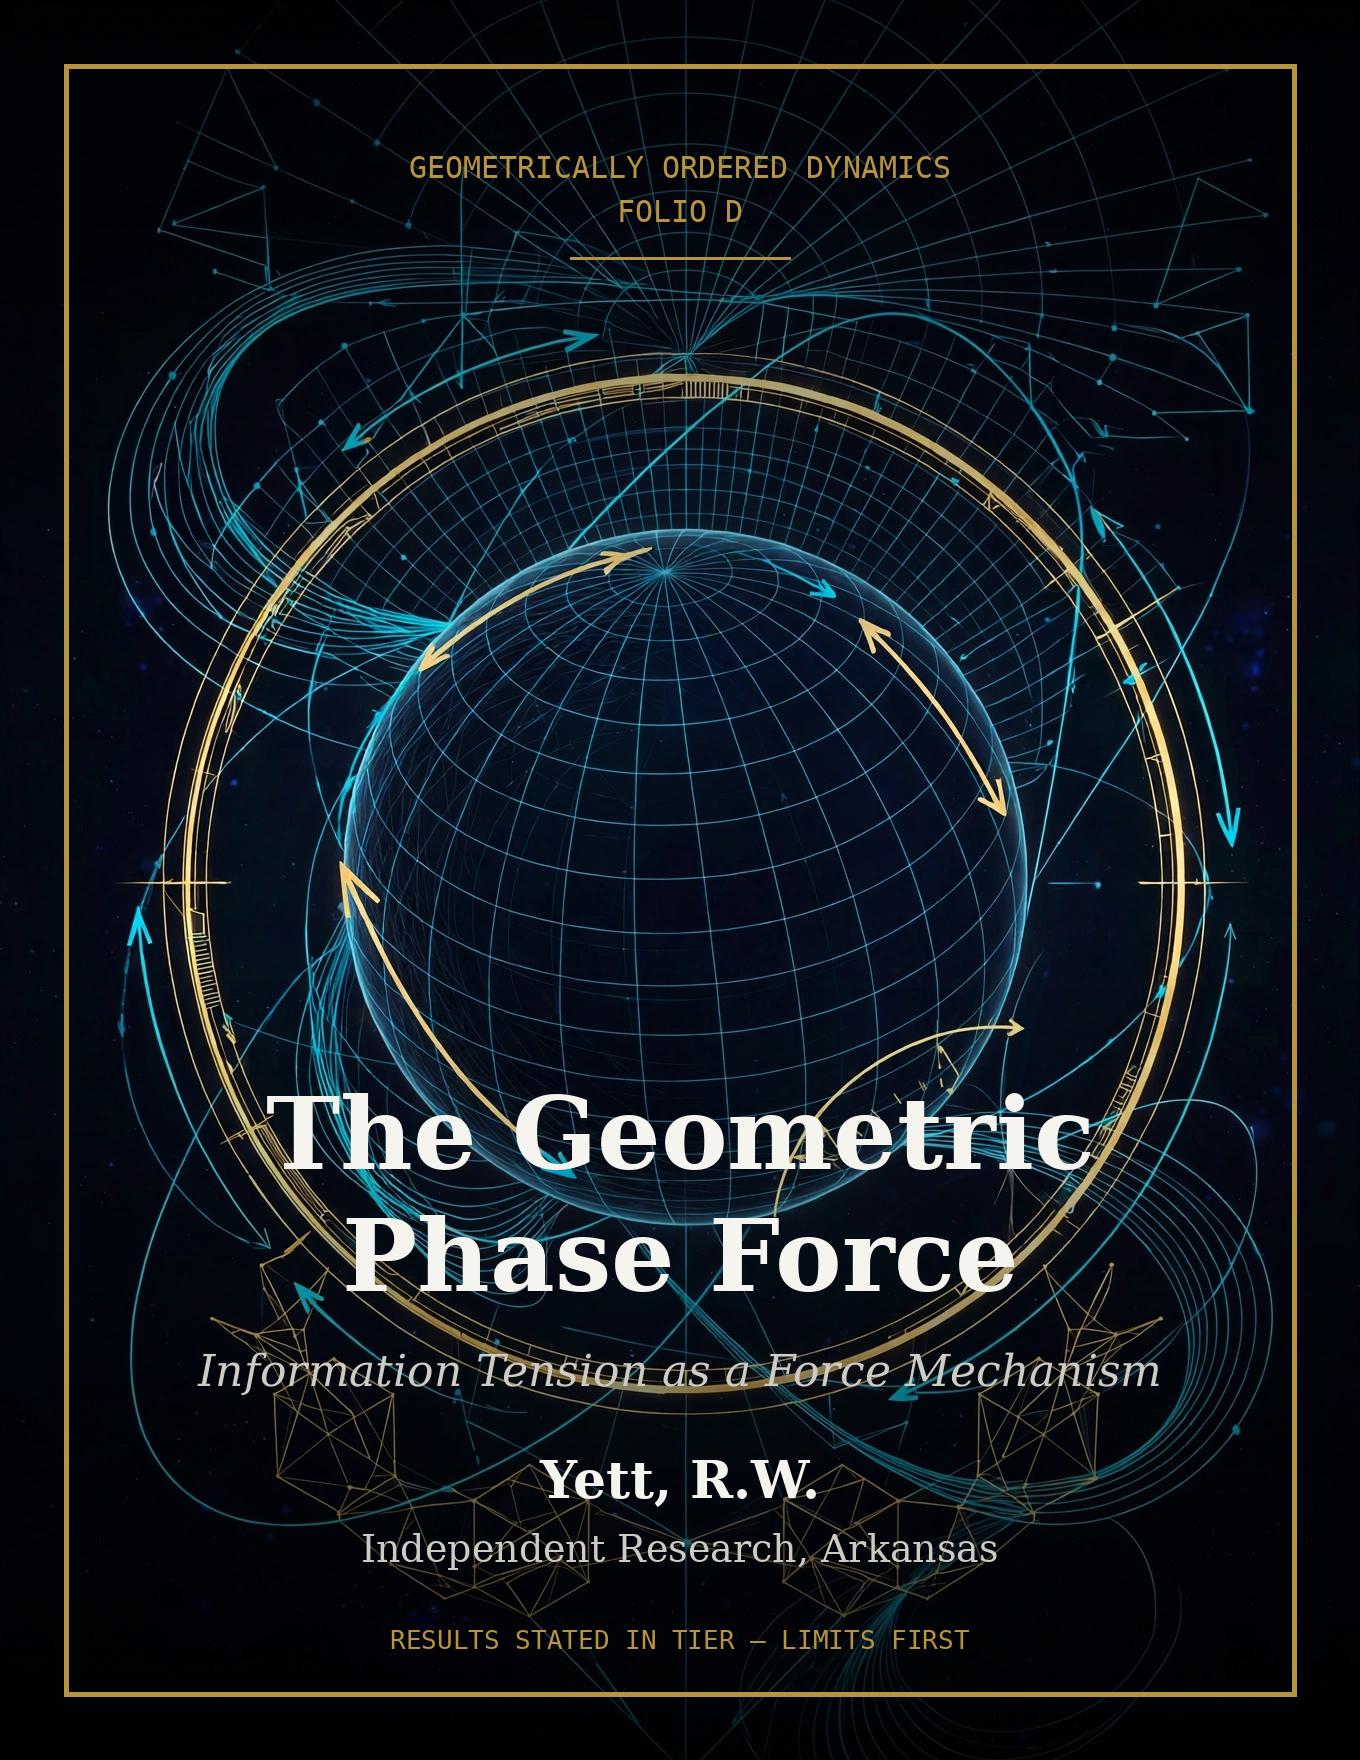
\includegraphics[width=\paperwidth,height=\paperheight]{cover.png}};
\end{tikzpicture}
\clearpage

\begin{convergence}{INFORMATION TENSION}
This folio converges on \key{information tension} as a geometric
force mechanism: the angle at which vacuum resistance to drift acts
like a force through a modified gravitational action. Its unique angle
is the \key{force mechanism} --- the Sovereign Action, the
information-tension tensor, and the horizon acceleration scale derived
from holonomy. Sibling papers approach the same claim from other
angles: \tiertag{conjecture} the geometric-foundation successor
(IT-FIELD companion) carries the foundations angle --- the scalar-tensor
action, the honest coupling statement, and the retracted empirics --- and
the Holonomery successor (IT-MARKET) carries the observer-substrate
angle of the same parallel-transport mathematics. Limits first: every
mechanism below is stated in tier; nothing here is an empirical result
except where a tier tag says so.
\end{convergence}

\begin{supersession}
This folio \textbf{supersedes} Zenodo record 20651497,
\textit{The Geometric Phase Force and the Sovereign Action} (and its
Drive predecessors \textit{quantum\_spearhead.pdf} and
\textit{prd\_horizon.pdf}), per the canon rule: the correction
\emph{becomes} the paper. Named repairs: (1) the abstract's claim that
``the entirety of these proofs has been subjected to mechanized
verification in Lean~4'' is withdrawn and replaced with the honest
formalization ledger (\S\ref{sec:formalization}); (2) the
Berry--Keating / Ramanujan-tau mass-gap identification is stated as
\tiertag{conjecture}, an un-discharged axiom, following the precedent
of the audit-corrected Ramanujan-Yett Hamiltonian v1.1 (Zenodo
21504896); (3) the five Clay Mathematics problem mappings are
re-stated as framework maps with named axioms, not solutions; (4) the
$T_2 \le 2T_1$ decoherence material keeps its honest tiering from
\textit{quantum\_spearhead}: the bound is textbook GKSL, the geometry
is conjecture; (5) the $a_0 = cH_0/2\pi$ horizon derivation from
\textit{prd\_horizon} is absorbed with its own stated O(1) gap and
limitations intact.
\end{supersession}

\section{The force mechanism}
\label{sec:mechanism}

The central loadbearing structure of the superseded record is the
\key{Sovereign Action} $S_Y$, a modification of the Einstein-Hilbert
action carrying a sovereign Lagrangian $\mathcal{L}_\chi$ and a
critical surface density $\Sigma_c$ linked to the geometric coherence
length $L_\chi = \hbar c / \Delta$:
\begin{equation}
S_Y = \int d^4x\,\sqrt{-g}\left[\frac{c^4}{16\pi G}R
+ \mathcal{L}_m
+ \alpha\left(\frac{\Sigma(r)}{\Sigma_c}\right)^2\right].
\end{equation}
Varying $\mathcal{L}_\chi$ with respect to the metric yields the
\key{information tension tensor} \tiertag{conjecture}:
\begin{equation}
\mathcal{T}_{\mu\nu} = \alpha\left(\frac{\Sigma(r)}{\Sigma_c}\right)
\left[g_{\mu\nu}\left(\frac{\Sigma(r)}{\Sigma_c}\right)
- \frac{4}{\Sigma_c}P_{\mu\nu}^{(\Sigma)}\right],
\end{equation}
the stress-energy of the $\chi$-field. The modified field equations
$G_{\mu\nu} = 8\pi G(1+f)T_{\mu\nu} + \cdots$ have legitimate
scalar-tensor form; the action shape is the honest mathematical core
of this folio. The 3rd-order radiation-reaction term carried by the
superseded record is retained as a modeling choice
\tiertag{conjecture}, not a derived necessity. No Ostrogradsky
stability proof is offered in this record.

\section{The low-acceleration limit}
\label{sec:lowacc}

Information tension stabilizes rotation curves in the low-acceleration
regime \tiertag{conjecture}. The superseded record's correction
$v_{\mathrm{yett}} = v_{\mathrm{newton}} \times T(r)$ produces the
MOND-like phenomenology stated cleanly: $\lim_{r\to\infty} v(r) =
\mathrm{const}$ for baryonic matter alone. This is the \key{force
mechanism} at work: as the surface density $\Sigma(r)$ drops, the
local chiral invariant $\chi$ approaches the 0.7 threshold and the
tension term rises to maintain the invariant, flattening the curve.
The phenomenological limit is loadbearing; the specific
$T(r) = 1.0 + (1.0/(\chi_{\mathrm{local}}\cdot 0.5))$ functional form
is a modeling choice, \tiertag{conjecture}, pending confrontation with
rotation-curve data in the companion foundation folio.

\section{The horizon acceleration scale}
\label{sec:horizon}

Absorbed from the Drive predecessor \textit{prd\_horizon.pdf}, with
its limitations intact. The MOND acceleration scale follows from a
geometric coherence identity \tiertag{conjecture}:
\begin{equation}
a_0 = \frac{cH_0}{2\pi},
\end{equation}
derived from the $\chi = 1/\sqrt{2} \equiv \cos(\pi/4)$ alignment bound
on Stiefel-manifold holonomy. Numerically $a_0 = 1.042 \times
10^{-10}\,\mathrm{m\,s^{-2}}$ (Planck $H_0$), within 13\% of the
empirical MOND value (6\% for local $H_0$); \textbf{no galaxy data
enters $a_0$}.

The derivation is grounded in three moves, two of them forced:
(i)~the connection is the acceleration, $A \sim a/c^2$, dimensionally
forced; (ii)~the loop is the cosmic-horizon great circle, the $2\pi$
geometrically forced; (iii)~the onset is the perturbative breakdown at
$|\oint A| = 1$, the standard strong-coupling criterion. The single
honest remaining gap, stated by the predecessor itself: the unity
threshold is \emph{motivated}, not uniquely forced from a deeper
principle --- one $O(1)$ convention stays open to external review.

\paragraph{Empirical status \tiertag{empirical}.} Tested against all
175 SPARC galaxies (3,389 radial points) with fixed stellar
mass-to-light ratios and zero fitted parameters, the parameter-free
law reproduces the Radial Acceleration Relation with median residual
$+0.04$~dex and rms $0.32$~dex, statistically indistinguishable from
MOND with empirical $a_0$ (reduced $\chi^2$ 88.6 vs 83.6). Stated
limitations, carried over: the 0.32~dex scatter exceeds the
marginalized literature RAR ($\sim$0.11~dex); lensing and the CMB
third peak remain open; the numerical coincidence $a_0 \sim
cH_0/2\pi$ is long noted (Milgrom 1983, 1999) --- the claim is the
derivation, not the number.

\section{The decoherence face}
\label{sec:decoherence}

Absorbed from the Drive predecessor \textit{quantum\_spearhead.pdf},
with its honest tier table intact. The GKSL master equation's Lindblad
jump operators are re-interpreted as gradients of the geometric
tension field, and the textbook bound $T_2 \le 2T_1$ is re-derived as
the non-negativity of the longitudinal tension-gradient variance
\tiertag{conjecture}. The tiering, stated by the predecessor and
preserved here:
\begin{itemize}
\item $T_2 \le 2T_1$ for physical qubits --- \tiertag{empirical}
standard GKSL, \emph{not} a novel prediction of this framework;
\item the machine-checked GKSL formalization (\texttt{Decoherence.\allowbreak lean},
zero sorry) --- \tiertag{theorem};
\item jump operators $= \nabla T$ --- \tiertag{conjecture},
geometric narrative;
\item absolute $T_1/T_2$ values from geometry --- not claimed;
\item spatial qubit-grid correlation falsifier --- \tiertag{conjecture}
open, see the Field Identity folio.
\end{itemize}
Passing the calibration-pair check proves consistency with Lindblad
complete positivity, nothing more.

\section{Formalization status: the honest ledger}
\label{sec:formalization}

The superseded abstract's sentence --- ``the entirety of these proofs
has been subjected to mechanized verification in Lean~4'' --- is
\textbf{withdrawn}. The honest status, per the Ars Magna correction
ledger (Zenodo 21277228): \textbf{13 Lean-verified modules} (E8 roots --- typed to the visible-sector factor of the E8$\times$E8 canon,
the spectral gap, $\zeta$-conjugation, $T_2 = 2T_1$, the nodal collar,
control-term trace preservation, and others) plus \textbf{3
axiom-carrying modules} whose named residuals are not discharged.
Everything beyond those modules is a \key{formalization scaffold},
not a mechanized proof. Any citation of this folio's formalism must
carry this ledger sentence with it.

\section{The spectral-gap identification}
\label{sec:spectralgap}

The identification of the Berry--Keating / Ramanujan-tau operator
structure with the Yang-Mills mass gap is stated as
\tiertag{conjecture}: an \textbf{un-discharged axiom}
(\texttt{yang\_\allowbreak mills\_\allowbreak gap\_\allowbreak equals\_\allowbreak stiefel\_\allowbreak gap}), following the
precedent of the audit-corrected Hamiltonian v1.1 (Zenodo 21504896).
The Stiefel spectral gap itself --- $H_{RY}$ self-adjoint, bounded
below, purely discrete spectrum with $\lambda_n - \lambda_0 \ge
\kappa^2 = 0.9099$ --- is \tiertag{theorem} (proof sketch; the Casimir
computation is not shown in-record). The \emph{identification} of that
gap with the Yang-Mills gap is the open axiom, not the theorem.

\section{Clay-class mappings as framework maps}
\label{sec:clay}

The superseded record's Table~7 mapped five Clay Mathematics problems
to ``resolutions.'' \textbf{Withdrawn as stated.} The honest form,
per the Ars Magna wording: these are \key{framework maps with named
axioms} --- ``framework solutions, not prize closures'':
\begin{itemize}
\item Yang-Mills: mass gap $\Delta$ mapped to the Lindblad/Stiefel
spectral gap; confinement via area law --- \tiertag{conjecture};
\item Navier-Stokes: global regularity conjectured via the
$\chi \ge 0.7$ threshold as Lyapunov function; $Re_c \approx 1.42$
is a dimensionless modeling number, not a derived critical value ---
\tiertag{conjecture};
\item Riemann Hypothesis: the critical line as sovereign gauge is a
stated analogy; ``off-line zeros rejected as hallucinations'' is
withdrawn as a claim --- \tiertag{conjecture};
\item P vs NP: complexity-as-information-tension is an analogy with no
exhibited map; no class separation is claimed --- \tiertag{conjecture};
\item Hodge: realizability via ADCCL condensation is asserted, not
proved --- \tiertag{conjecture}.
\end{itemize}
Each mapping names the axiom it would need; none is discharged.

\section{What this folio claims and does not claim}

\key{Claims:} a scalar-tensor action shape with an honestly stated
formalization ledger (\S\ref{sec:formalization}); a conjectured force
mechanism flattening rotation curves in the low-acceleration limit
(\S\ref{sec:lowacc}); a derived-but-$O(1)$-open horizon acceleration
scale with an empirical SPARC test (\S\ref{sec:horizon}); a tiered
decoherence reinterpretation (\S\ref{sec:decoherence}); conjectured
framework maps to five Clay-class problems with named open axioms
(\S\ref{sec:clay}). \key{Does not claim:} mechanized verification of
the whole (\S\ref{sec:formalization}); any empirical dataset of its
own --- the Trinity 2.0 empirics are retracted corpus-wide and are
not cited here; a solution to any Clay Mathematics problem.

\goldrule

\paragraph{References.} Superseded: \doi{10.5281/zenodo.19835025}
(record 20651497; the DOI printed on its own cover). Honesty
standards: \doi{10.5281/zenodo.21277228} (Ars Magna correction
ledger); \doi{10.5281/zenodo.21504896} (Ramanujan-Yett Hamiltonian
v1.1, audit-corrected). Data: SPARC (Lelli, McGaugh \& Schombert
2016, \textit{AJ} \textbf{152}, 157); Milgrom (1983, \textit{ApJ}
\textbf{270}, 365). Prior art note: the $a_0 \sim cH_0/2\pi$
coincidence is Milgrom's (1983, 1999); the derivation claim is the
novel content.

\end{document}
